\documentclass[UTF8,journal,twoside,web]{ieeecolor}
\usepackage{ctex}
\usepackage{generic}
\usepackage{cite}
\usepackage{amsmath,amssymb,amsfonts}
\usepackage{graphicx}
\usepackage{textcomp}
\usepackage{booktabs}
\usepackage{threeparttable}
\usepackage{algorithm}
\usepackage{algorithmic}
\usepackage{titlesec}
\usepackage{makecell}
\usepackage{subfig}
\usepackage{float}
\usepackage{stfloats}
\usepackage{adjustbox}
% \usepackage{color}
\renewcommand{\algorithmicrequire}{\textbf{输入：}}  % 使用算法格式中的 Input
\renewcommand{\algorithmicensure}{\textbf{输出：}} % 使用算法格式中的 Output

\newcommand{\newtext}[1]{{\leavevmode\color{blue}#1}}

% \abovedisplayshortskip=6pt
% \belowdisplayshortskip=6pt
% \abovedisplayskip=6pt
% \belowdisplayskip=6pt

% \titlespacing\section{0pt}{12pt plus 4pt minus 2pt}{0pt plus 2pt minus 2pt}
% \titlespacing\subsection{0pt}{12pt plus 4pt minus 2pt}{0pt plus 2pt minus 2pt}
% \titlespacing\subsubsection{0pt}{12pt plus 4pt minus 2pt}{0pt plus 2pt minus 2pt}

% \setlength{\abovecaptionskip}{0pt}
% \setlength{\belowcaptionskip}{0pt}

\makeatletter
\newcommand{\removelatexerror}{\let\@latex@error\@gobble}
\makeatother

\begin{document}
\title{用于工业应用中电池健康状态可信估计的分层随机时空 Transformer
% \vspace{-1em}
}
\maketitle
\begin{abstract}
随着锂离子电池在安全关键行业的广泛应用，对电池健康状态进行准确可靠的估计（称为可信预测）已变得至关重要。然而，在代表性相关学习过程中忽视模型不确定性可能导致对模糊段的不恰当聚合。此外，主导空间通道的偏移和有用时间特征的稀疏性进一步阻碍了可信估计。再者，预测分布与实际分布之间的不对齐导致置信度偏差问题，并降低了区分分布外样本的性能。为解决这些挑战，本文提出了一种分层随机时空 Transformer（HSSTT）。首先，HSSTT 利用 Gumbel-Softmax 重参数化实现随机自注意力以进行不确定性量化。然后，设计了一种分层时空 Transformer，利用不确定性感知的时间步扩展卷积和聚类随机自注意力。最后，本文通过偏差-方差分解从理论上分析了置信度偏差问题，并提出了一种有原则的校准策略。在四个数据集上针对七种最先进模型的实验结果证明了 HSSTT 在可信预测方面的优越性。
\end{abstract}

\begin{IEEEkeywords}
锂离子电池, 健康状态估计, 不确定性量化, 不确定性校准.
\end{IEEEkeywords}

\section{引言}\label{sec:introduction}

锂离子电池（Lithium-ion Batteries, LIBs）凭借其优越的功能特性，在工业领域得到了广泛的应用，尤其是作为电动汽车动力电池\cite{NASAJPOURESFAHANI2024114783, hannan2017review}。然而，严苛的工业环境与复杂的内部电化学反应相叠加，亟待采取更为严密的保障措施，以确保LIBs长期的安全与可靠运行。因此，对LIBs的性能进行有效监测以保障其持续稳定运转显得尤为关键。通常而言，电池的性能由 SOH 表征，该指标被定义为电池当前最大可用容量与其标称容量之比\cite{WANG2024110325, 10391265}。

深度学习的蓬勃发展极大地推动了数据驱动 SOH 估计模型的涌现。此类模型极大降低了模型开发过程对领域专家知识的依赖，并在捕捉复杂退化机制动态特性方面展现出卓越能力，因而正逐步取代传统的基于物理的模型\cite{mit_dataset_attia2020closed, tri_dataset_severson2019data, tongji_dataset_zhu2022data}。然而，工业环境中不可避免的噪声波动与多变的负载需求，往往导致样本数据呈现出复杂且难以解析的分布特征；在处理此类样本时，数据驱动模型依然极易产生不准确的估计结果\cite{10214203}。此外，受限于其确定性本质，此类模型仅能提供SOH的单一“点估计”，而缺乏对潜在误差的预警能力，如图~\ref{fig:hsstt_challenges}(a) 所示。过度依赖此类确定性模型势必会对后续的决策过程带来风险。例如，若 LIBs 的 SOH 估计值低于实际值，将导致电池提前退役，进而造成不必要的经济损失；反之，若高估SOH，则会引发电池的过度循环使用，从而增加系统级热失控的潜在风险。

为规避确定性模型引发的潜在问题，并切实保障工业级监测与维护的可靠性，对数据驱动预测模型输出结果的可信度进行评估显得至关重要。鉴于其与高可信 SOH 估计之间的紧密联系，不确定性的量化被认为居于核心地位\cite{THUY2024330, 10539360}。一方面，不确定性可作为一种量化测度，通过衡量模型表征的概率分布与真实分布之间的偏差，客观地反映出估计结果的可信程度；另一方面，不确定性亦可作为一种以用户为导向的可靠性分析指标，能够自然融入涉及人工干预的实际决策流程之中。综上，实际工业应用对 LIBs 的高可信预测模型提出了迫切需求，而在构建此类模型时，仍面临着以下需要解决的问题：

（1）表征关联学习过程中的不确定性构成了第一项挑战。在关联信息聚合阶段，模型生成权重分数时所固有的不确定性被忽略。某些本不重要且可能具有高不确定性的循环信号片段易被错误地分配较高的权重值 \cite{20222012122312, 20191806851746, 10342686}。如图~\ref{fig:hsstt_challenges}(a) 所示，对这些冗余信号片段的过度聚合，将误导对复杂退化动态特征的提取，最终导致 SOH 估计精度的降低。

（2）对时空不确定性的忽视构成了第二项挑战。针对 LIBs 的循环充放电信号，主导通道的变动会导致跨传感器依赖关系发生波动，进而引发传感器数据融合过程中的不一致性。与此同时，跨时间依赖关系的稀疏分布特征，亦为提取信号片段对之间的交互特征引入了模糊性。如图~\ref{fig:hsstt_challenges}(a) 所示，若未能对此类时空不确定性进行充分且有效的建模，估计结果的精度亦将降低 \cite{wang2023inherent, 9729404, capsnet_rul_li2024sensor}。

（3）不确定性的潜在校准失真构成了第三项挑战。在实际应用场景中，原始数据的真实分布难以解析，导致通过不确定性量化所导出的预测分布可能与真实分布存在严重偏差 \cite{kuleshov2018accurate, 9729404, 10217044}。如图~\ref{fig:hsstt_challenges}(b) 所示，这种分布差异直接引发了区间估计的过度自信或置信度不足问题。其结果不仅削弱估计结果的可信度，同时损害看了基于不确定性分数的分布外检测性能。

为应对上述挑战，本文提出一种层次化随机时空 Transformer（Hierarchical Stochastic Spatial-Temporal Transformer, HSSTT）。在 HSSTT 中，设计一种基于 Gumbel-Softmax 重参数化（Gumbel-Softmax Reparameterization, GSR）的自注意力机制。该机制将传统的确定性自注意力转化为随机自注意力，旨在处理特征提取与特征映射过程中的不确定性。随后，结合具有不确定性量化能力的膨胀时间步卷积与上述随机自注意力机制，以充分提取跨传感器的空间退化动态特性与跨循环的时间退化动态特性。最后，通过偏差-方差分解解释模型过度自信或置信度不足的成因，并据此构建模型无关的校准策略；通过利用校准后的不确定性，模型能够精准区分分布内（ID）与分布外（OOD）样本。HSSTT 的贡献如下：

（1）提出了一种全新的随机自注意力机制，其利用 GSR 赋予自注意力以不确定性量化能力，为高可信 SOH 估计提供支撑。

（2）以不确定性为导向进行时空依赖性建模与退化动态提取，消除了循环数据中的模糊性，从而提高模型 SOH 估计性能。

（3）阐明模型校准失真成因，提出了一种模型无关的不确定性校准方法以精准拟合实际数据分布，并验证了将校准得到的无偏不确定性应用在分布外退化模式检测中的潜力。

（4） 在 4 个公开数据集上开展了详尽的综合实验。实验结果充分证实了 HSSTT 在可信 SOH 估计任务中的有效性与先进性。

\begin{figure}[!t]
  \centering
  \includegraphics[width=3.4in]{figures/figure1/problem_formulation_revised.eps}
  \caption{(a) 确定性模型、(b) 具有不确定性但未校准的模型以及 (c) 可信模型提供的 SOH 估计结果示意图。}
  \label{fig:problem}
  % \vspace*{-0.5em}
  \end{figure}

% 第一个挑战源于代表性相关学习过程中的不确定性。
首先，代表性相关学习过程中的不确定性构成了一个挑战。
在聚合相关信息的过程中，模型在生成权重 logit 时的不确定性常常被忽视。一些不重要的 token，可能表现出高不确定性，可能被错误地分配高 logit\cite{20222012122312, 20191806851746, 10342686}。如图~\ref{fig:problem}(a) 所示，聚合这些不重要的 token 可能误导复杂退化动态的提取，最终降低 SOH 估计结果的精度。

% 第二个挑战是忽视时空不确定性。
其次，忽视\newtext{时空不确定性}构成了一个挑战。
对于 LIBs 的循环信号，由于主导通道偏移导致的跨传感器依赖性变化可能导致传感器数据融合的不一致。同时，跨时间依赖性的稀疏分布增加了 token 对交互提取的模糊性。对这种时空不确定性的不充分建模会损害预测精度\cite{wang2023inherent, 9729404, capsnet_rul_li2024sensor}，如图~\ref{fig:problem}(a) 所示。

% 第三个挑战是不确定性的潜在校准错误。
第三，不确定性的潜在校准错误构成了一个挑战。
在应用中，实际数据分布是不可访问的，通过量化不确定性导出的预测分布可能与实际分布不一致\cite{kuleshov2018accurate, 9729404, 10217044}。如图~\ref{fig:problem}(b) 所示，这导致置信度不足或过高的区间估计。结果，预测结果的可信度降低，基于不确定性分数的分布外样本检测性能下降。

为解决这些问题，本文提出了一种\textbf{分}层\textbf{随}机\textbf{时}\textbf{空} \textbf{Transformer}（HSSTT）。在 HSSTT 中，设计了一种新颖的基于 Gumbel-Softmax 重参数化（GSR）的自注意力机制，将确定性自注意力转化为其随机对应物，以处理特征提取和特征映射过程中的不确定性。然后，开发了一种分层随机时空 Transformer，结合不确定性感知的时间步扩展卷积和随机自注意力，以提取跨传感器（空间）和跨循环（时间）的退化动态。最后，通过偏差-方差分解分析了模型置信度不足或过高的原因，在此基础上制定了一种有原则的校准策略，并利用校准后的不确定性来区分分布内（ID）和分布外（OOD）样本。主要贡献如下。

\begin{enumerate}
  \item 我们提出了一种利用 GSR 实现具有不确定性量化能力的自注意力机制的随机自注意力机制。此外，随机自注意力作为 HSSTT 的基本组件，用于可信的 SOH 估计。
  \item 我们提出了一种分层随机 Transformer，通过不确定性引导的时空依赖性建模和退化动态提取，从而消除循环数据中的模糊性并增强预测性能。
  \item 我们分析了模型校准错误的原因，并提出了一种针对 HSSTT 的有原则校准方法，以更好地建模实际数据分布。基于无校准偏差的的不确定性，我们设计了一种针对预测场景的 OOD 检测策略。
  \item 我们在三个公开数据集上进行了全面的实验来评估 HSSTT 的性能，实验结果证实了 HSSTT 在可信 SOH 估计方面的有效性和优越性。
\end{enumerate}

本文的其余部分组织如下。所提出的预测模型 HSSTT 在第~\ref{sec:methodology} 节中详细介绍。第~\ref{sec:experiment} 节展示了全面的实验，以证明 HSSTT 的 SOH 估计、不确定性量化和不确定性校准结果。第~\ref{sec:conclusion} 节得出结论。

\begin{figure*}[h]
  % \vspace{-1.5em}
  \centering
  
\includegraphics[width=6in]{figures/figure2/framework.pdf}
  % \vspace{0.5em}
  \caption{HSSTT 的框架。该框架包含不确定性感知随机自注意力（"opt." 子模块专门用于时间依赖性提取）、分层时空特征提取模块以及有原则的不确定性校准机制。}
  \label{fig:framework}
  \end{figure*}

\section{相关工作}\label{sec:related_works}

在本节中，我们回顾与不确定性感知预测相关的方法，将其分为两类范式：基于物理的模型和数据驱动模型。

\subsection{基于物理的不确定性感知预测模型}\label{subsec:physics-based_models}

基于物理的预测模型通过将退化机制与用于状态估计和参数更新的滤波技术相结合来推导具有不确定性意识的预测。所使用的滤波器——主要是卡尔曼滤波器和粒子滤波器——利用固有的贝叶斯框架，通过对系统状态和噪声分布进行概率推理来量化不确定性\cite{chen2003bayesian}，从而实现对预测结果的动态置信区间估计。
% 2016
Bressel 等人\cite{7386653} 提出了一种基于扩展卡尔曼滤波器的算法，结合一阶逆可靠性方法进行 SOH 和剩余使用寿命（RUL）预测，以及相应的置信区间。
% 2021
Kim 等人\cite{9032349} 提出了一种利用动态粒子滤波的预测模型，量化与电池寿命终止相关的不确定性，并自适应调整退化模型的参数。
% 2021
Haque 和 Choi\cite{9113648} 提出了一种利用稀疏核岭回归辅助粒子滤波的预测模型，通过考虑噪声不确定性来量化退化轨迹的突然变化。
% 2022
Ahwiadi 和 Wang\cite{AHWIADI2022110817} 提出了一种基于进化模糊预测器的增强粒子滤波模型，以缓解样本退化和贫乏问题，同时实现高精度的剩余使用寿命区间估计。
% 2023
Rezaei 等人\cite{REZAEI2023107883} 开发了一种模糊鲁棒两阶段无迹卡尔曼滤波器，使用噪声协方差矩阵分阶段估计循环容量和量化不确定性。
% 2024
Cui 等人\cite{10385053} 设计了一种基于双无迹粒子滤波的预测模型，以解决动态退化轨迹中的不确定性并实现鲁棒预测。
% 2024
Wang 等人\cite{10672556} 提出了一种基于区间卡尔曼滤波器的方法，带有物理约束，以实现在线容量区间估计。


\subsection{基于数据驱动的不确定性感知预测模型}\label{subsec:data-driven_models}

基于数据驱动的不确定性感知预测模型可分为基于统计学习的方法\cite{van2021bayesian, gruber2025sourcesuncertaintysupervisedmachine}和基于深度学习的方法\cite{ABDAR2021243}。统计学习方法依赖显式概率模型进行分析或近似推理。相比之下，深度学习方法通过利用随机化参数空间或输出分布的统计特性来解决不确定性问题。
% 
Wang 等人\cite{rvr_rul_9552552} 介绍了一种基于相关向量回归（RVR）的预测方法，而
Richardson 等人\cite{gpr_soh_8263147} 采用高斯过程回归（GPR）进行 SOH 估计。
% 
Zhang 等人\cite{bbb_rul_9738999} 开发了一种贝叶斯混合神经网络（BMNN）来捕获预测结果的分布。
%
Li 等人\cite{capsnet_rul_li2024sensor} 提出了一种基于 dropout 的剩余使用寿命（RUL）预测框架，名为 SACN。
%
Zhang 等人\cite{ensemble2_soh_10102497} 结合多模型融合方法和深度集成神经网络来量化 SOH 估计不确定性，称为 DeNN。
%
Zhou 等人\cite{mcdropout_autoencoder_10412192} 设计了一种带有蒙特卡洛 dropout（MCD）和变分推理的贝叶斯深度自编码器（BDAE），用于测量 SOH 估计中的不确定性。
%
Nemani 等人\cite{nemani2023uncertainty} 提出了一种专注于谱归一化神经高斯过程（SNGP）的策略，用于确定性不确定性量化。
%
Lin 和 Li\cite{9729404} 介绍了一种利用 Concrete Dropout 进行 RUL 预测的贝叶斯神经网络（BNN）框架，其中通过结合等渗回归和标准差（STD）缩放集成了迭代校准。
%
Ke 等人\cite{10217044} 开发了一种基于 MCD 的 BNN 模型，用于 LIBs 的拐点容量预测，并使用 STD 缩放方法进行不确定性校准。
%
Jiang 等人\cite{10391265} 提出了一种基于 Bayes-by-Backprop 策略的神经网络，带有不确定性校准，用于估计梯次利用电池的 SOH。

尽管取得了进展，但在提供既高度准确又无偏差的预测结果方面仍存在一些开放性问题。
% 
首先，基于物理的模型主要关注噪声引起的不确定性，导致模型置信度表示不足和结果不一致。相反，数据驱动模型中的那些缺乏粒度和结构适应性，阻碍了退化模式的有效提取。
% 
其次，现有关注 SOH 预测中模型不确定性的方法往往忽视数据中的时空不确定性。这可能导致在退化建模中使用不相关或错误的数据段，从而降低预测精度。
% 
第三，由于其近似性质，不确定性感知预测模型可能无法充分表示循环数据的实际分布。即使在估计值与实际值存在显著偏差时，它们也表现出较小的不确定性，从而无法区分 ID 和 OOD 样本。
% 
为解决上述问题，我们提出了 HSSTT，一种利用不确定性建模并结合校准过程的可信 SOH 估计方法，以增强注意力聚合和时空退化依赖性提取。


\section{方法}\label{sec:methodology}

在本节中，我们详细阐述所提出的 HSSTT 框架，深入分析 HSSTT 在实际工业场景中的部署，并详细介绍实现可信 SOH 估计的方法。如图~\ref{fig:framework} 所示，token 之间的相关性信息通过所提出的随机自注意力进行聚合。退化动态通过设计的不确定性感知时空特征编码器捕获，并通过下游回归器映射到 SOH。模型不确定性采用蒙特卡洛采样进行量化，并通过所提出的有原则辅助模型进一步校准。

\subsection{用于不确定性量化的随机自注意力}\label{subsec:stochastic_attention}

为解决由于忽视模型不确定性而导致的合并模糊段的问题，我们提出了一种基于 Gumbel-Softmax 重参数化（GSR）技术的不确定性感知自注意力机制。这种创新的自注意力机制是构建 HSSTT 最基础和最核心的组件。

基于 Transformer 的模型的卓越上下文建模能力主要归因于多头自注意力（MHA）机制。以第 $j$ 个头为例，序列 $X=[x^{(1)}, x^{(2)}, \ldots, x^{(T)}] \in \mathbb{R}^{d_{in} \times T}$ 通过可训练的投影矩阵 $W_{Q}^{(j)}, W_{K}^{(j)}, W_{V}^{(j)} \in \mathbb{R}^{d_{emb} \times d_{in}}$ 进行仿射变换，生成查询 $Q^{(j)}$、键 $K^{(j)}$ 和值 $V^{(j)}$。这里，$T$ 是每个序列样本中的总循环次数，而 $d_{in}$ 和 $d_{emb}$ 分别是输入和嵌入的维度。

由 softmax 函数产生的注意力权重 $A^{(j)}$ 表现出离散概率分布的形式，表明它们可以被视为从分类分布中采样\cite{20193407356730, 20230613569727}。通过用 Gumbel-Softmax 替代 softmax 并将确定性计算替换为概率采样方法，我们将自注意力转化为其随机对应物。这种修改将每个 token 的注意力权重改变为具有几个离散结果的分类分布，可表示为
\begin{equation}
% \tilde{A}^{(j)}\sim\mathcal{G}(\frac{K^{(j)^\top}Q^{(j)}}{\tau})
\tilde{A}^{(j)}\sim\mathcal{G}((K^{(j)^\top}Q^{(j)}) / \tau),
\label{eq:gumbel-softmax-attention}
\end{equation}%
其中 $\mathcal{G}$ 是 Gumbel-Softmax 函数，$\tau$ 是温度参数。因此，通过自注意力机制导出的注意力权重 $\tilde{A}^{(j)}$ 从特定的归一化 logit 转变为从不同的离散分布中概率采样的随机变量。通过这种方式，确定性自注意力被转化为用于不确定性量化的随机变体。

随机自注意力构建的基础是离散分类分布的连续松弛，这可以通过 GSR 技术有效实现。考虑一个非负离散分类分布 $(\pi_{1},\pi_{2},\cdots,\pi_{T})$，不完全为零，表示自注意力中特定 token 的注意力权重。具体而言，$\pi_{i}=k_{i}^\top q_{i}$ 表示矩阵 $K^{(j)}$ 和 $Q^{(j)}$ 的列划分结果，其中 $i$ 表示列索引。第一步涉及检查该分布的索引变量，表示为
\begin{equation}
z=one\_hot(argmax(g_{i}+\log(\pi_{i}))),
\label{eq:index_variable}
\end{equation}%
其中 $T$ 是离散分类分布中可能结果的总数，对应于输入 token 的数量。此外，$g_i$ 是一个服从 $Gumbel(0,1)$ 分布的随机变量，表示为
\begin{equation}
g_{i}=-\log(-\log(u_{i})),
\label{eq:gumbel_noise}
\end{equation}%
其中 $u_i$ 在 0 和 1 之间均匀分布，$g_i$ 和 $u_i$ 都是独立同分布（i.i.d.）的简单随机样本，$g_i$ 也称为 Gumbel 噪声。\eqref{eq:index_variable} 中的 argmax 操作是不可微的，因此采用 GSR 技术将其转化为连续的对应物，得到
\begin{equation}
\tilde{A}^{(j)}=\frac{\exp((g_{i}+\log(\pi_{i}))/\tau)}{\sum\nolimits_{k=1}^{T}\exp((g_{i}+\log(\pi_{k}))/\tau)},
\label{eq:gsr_relaxation}
\end{equation}%
这等价于 \eqref{eq:gumbel-softmax-attention}。在 MHA 的上下文中，$\tau$ 用作原始缩放因子 $1 / \sqrt{d_{emb}}$ 的替代品。从 GSR 的角度来看，上述等式的右侧近似于离散分类分布 $(\pi_{1}, \pi_{2}, \cdots, \pi_{T})$。当 $\tau$ 趋向于零时，Gumbel-Softmax 分布越来越类似于原始分类分布。采用 GSR 技术进行连续松弛将不可微的分类分布转化为平滑、可微的 GS 分布。这种变换允许直接应用反向传播来训练随机自注意力。最初，$\tau$ 被设置为相对较大的值，随着模型在训练过程中趋向收敛而逐渐减小，从而优化速度和有效性之间的平衡。

显然，GSR 技术通过将 Gumbel 噪声纳入 logit 来生成注意力权重，然后对所得向量应用 softmax 函数。如\cite{potapczynski2020invertible} 中详细所述，Gumbel 和高斯噪声之间存在直接映射，确保基于 GSR 的方法和 MCD 等方法在根本上是一致的。我们在第~\ref{subsec:ablation_study} 节中呈现的实证发现证明，所提出的方法在捕获模型不确定性方面优于基于 MCD 的方法。

\newtext{从确定性注意力机制到随机注意力机制的转变为观察模型内部决策过程提供了一个直接的窗口，这不仅提供了量化不确定性的关键优势，还提供了模型可解释性。将注意力权重概念化为分布，使得其在多次随机前向传递中的方差可以作为模型对每个输入 token 显著性信心的可量化指标。低方差表明对特征作为稳定退化指示器效用的信心很高。相反，高方差表示在遇到噪声或模糊数据段时模型的不确定性。这种固有的可解释性有助于在输入数据上生成"不确定性图"，为随后详细介绍的基于可信度的特征提取过程提供基础。}

\subsection{基于分层随机 Transformer 的时空编码器}\label{subsec:hierarchical_spatialtemporal}

\newtext{受分层时空建模\cite{qianhstformerhierarchicalspatialtemporaltransformers}和概率 Transformer\cite{9879185}并行进展的启发，我们设计了一种基于分层随机 Transformer 的时空编码器，统一了这些原理，解决了电池退化建模固有的复杂性和可信性双重挑战。}
% 
首先，实现了一种不确定性感知扩展卷积用于空间信息提取，产生跨传感器依赖性感知的嵌入。然后这些嵌入由随机距离敏感 Transformer 编码器进行时间建模处理，其中设计了一种聚类机制来处理特征稀疏性并形成分层 Transformer。

我们提出了一种简单而有效的方法，利用不确定性感知时间步卷积来挖掘跨传感器依赖性。这种技术应用于在第 $t$ 个循环期间从 $S$ 个传感器收集的长度为 $L$ 的多变量时间序列数据 $r^{(t)} \in \mathbb{R}^{S \times L}$，具有几个关键特征：1）它采用扩展卷积来扩大感受野，从而识别不同时间步不同传感器之间的潜在相关性；2）它采用随机自注意力通过不确定性重新加权注意力来识别主导传感器通道；3）卷积核的水平分量大于 1 以检测跨传感器依赖性；4）卷积生成的特征图随后被展平为列向量，作为样本 $X_{i}$ 的时间步特定组件。卷积后，$r^{(t)}$ 被转换为 $x^{(t)} \in \mathbb{R}^{d_{in} \times 1}$。

同时，退化动态的时间表示通过自注意力实现。Vanilla Transformer 的正弦位置嵌入可能导致忽视 SOH 估计的循环实例之间关键距离。受\cite{wu-etal-2021-da} 启发，我们通过直接修改随机自注意力权重 $\tilde{A}^{(j)}$ 来纳入 token 之间的真实距离信息。对于给定的时间序列 $X$，任意两个 token 位置 $p$ 和 $q$ 之间的距离定义为 $r_{p,q} = |p-q|$，创建距离矩阵 $R = (r_{p,q}) \in \mathbb{R}^{T \times T}$。此外，为 MHA 中的每个头分配一个可学习参数 $\omega$ 以动态调整距离敏感度。关注第 $j$ 个头，其特定距离矩阵 $R^{(j)} = \omega^{(j)}R$ 允许区分长期和短期信息，正值的 $\omega$ 有利于前者，负值有利于后者。为了将此加权距离矩阵 $R$ 与自注意力无缝合并，使用动态 sigmoid 函数将 $R$ 投影到重新缩放的系数上，其公式为
\begin{equation}
% \hat{R}^{(j)}=f(R^{(j)},V^{(j)})=\frac{1+\exp(V^{(j)})}{1+\exp(V^{(j)}-R^{(j)})}
\hat{R}^{(j)} = \frac{1+\exp(V^{(j)})}{1+\exp(V^{(j)}-R^{(j)})},
\label{eq:distance_matrix_coefficient}
\end{equation}%
其中 $V^{(j)}$ 是第 $j$ 个头的可训练参数，调节 sigmoid 函数的上限和上升陡度。然后我们用 $\hat{R}^{(j)}$ 来调整 \eqref{eq:gumbel-softmax-attention} 中概述的随机注意力权重，修改后的注意力权重矩阵公式为
\begin{equation}
% \hat{A}^{(j)} \sim \mathcal{G}\left(\frac{\sigma({K^{(j)}}^\top Q^{(j)}) * \hat{R}^{(j)}}{\tau}\right)
\hat{A}^{(j)} \sim \mathcal{G}((\sigma({K^{(j)}}^\top Q^{(j)}) * \hat{R}^{(j)}) / {\tau}),
\label{eq:distance_sensitive_self_attention}
\end{equation}%
其中 $*$ 是 Hadamard 积，$\sigma$ 是激活函数，选择 ReLU 函数以确保非负性。

为了促进模型在稀疏特征空间中有效提取与老化状态相关的健康特征，同时不受多余或无关信息的影响，设计了一种分层随机自注意力机制，其灵感来自\cite{clustered_attention_vyas2020fast}。该机制在采样注意力权重之前对键头进行聚类，等价于对键注意力头进行正则化，并强制模型关注预定义的稀疏聚类质心。通过用 Gumbel-Softmax 替代 softmax，近似质量分析的完整性仍然得到保证。这确保了聚类前后键注意力之间的差异保持有界。基于此，我们选择了一种新颖的方法来替代\cite{clustered_attention_vyas2020fast} 中建议的 Hamming 空间中 \textit{k}-means 聚类的 Lloyd 算法。我们的方法涉及将质心矩阵视为可训练矩阵，随着模型趋向收敛，促进高效的 optimal 聚类划分。此外，分层机制将自注意力的二次计算复杂度降低为线性形式\cite{clustered_attention_vyas2020fast}，从而缓解变分推理引起的计算负担并提高模型的响应速度。

这种分层随机距离敏感自注意力机制的公式为
\begin{align}
\label{eq:attention_kqv} & Q^{(j)}, K^{(j)}, V^{(j)} = W_{Q}^{(j)}X, W_{K}^{(j)}X, W_{V}^{(j)}X, \\
\label{eq:hsstt_k} & \hat{A}_{C} \sim \mathcal{G}(({K^{(j)}}^\top C) / \tau_{1}), \\
\label{eq:hsstt_clustered_k} & \hat{K}^{(j)} = \hat{A}_{C}C^\top, \\
\label{eq:hsstt_hierarchical_attention} & \hat{A}^{(j)} \sim \mathcal{G}((\sigma(\hat{K}^{(j)\top} Q^{(j)})*\hat{R}^{(j)}) / \tau_{2}), \\
\label{eq:hsstt} & \hat{H}^{({j})}=\hat{A}^{({j})}V^{{(j)}}, \\
\label{eq:hsstt_mha} & \widehat{MHA}=concat(\hat{H}^{(1)},\hat{H}^{(2)},\cdots,\hat{H}^{(h)})W_{O},
\end{align}%
其中 $C \in \mathbb{R}^{d_{emb}\times C}$ 是质心集合，$\hat{A}_{C}$ 是从 Gumbel-Softmax 分布采样的质心权重，$\hat{K}^{(j)}$ 是聚类后的键头，$\tau_{1}$ 和 $\tau_{2}$ 是温度系数，$h$ 是头数，$W_{O} \in \mathbb{R}^{h \times d_{emb} \times d_{in}}$ 是可训练投影矩阵。获取电池退化模式的表示后，采用由多个全连接层组成的回归器将这些特征图映射到 SOH 估计值。

\newtext{这种不确定性引导的原理支配着编码器的操作。模型学会动态地将注意力资源分配给表现出高置信度的特征。该机制在空间和时间域中实现。不确定性感知卷积和随机 Transformer 都学会减弱高方差特征的影响，抑制来自噪声传感器通道和模糊时间段的贡献。这样的过程产生了对无关信息具有鲁棒性的特征表示。SOH 估计的最终预测不确定性来自这些局部化内部不确定性的聚合。因此，模型对其特征选择的信心直接转化为其最终预测的信心，将模型的推理过程与其输出的可信度联系起来。}

\subsection{面向良好校准的 HSSTT}\label{subsec:uncertainty_calibration}

为获得准确可靠的不确定性估计并增强 HSSTT 的可信度，我们研究了不确定性校准问题。首先，我们从偏差-方差分解的角度理论上分析模型置信度不足或过高的原因，并强调不确定性校准的重要性。随后，我们提出了一种有原则的校准策略，将 HSSTT 的预测不确定性与从数据样本导出的经验不确定性对齐。

经验观察表明，现有的不确定性感知方法呈现出二元趋势：表现出较高预测精度的模型以置信度偏差量化不确定性，而提供高质量不确定性量化的模型精度较低。我们使用偏差-方差分解从理论上分析这一现象，其公式为
\begin{align}
\label{eq:bias_variance_tradeoff} & E((y-\hat{f}(X))^{2}) = Bias^{2}(\hat{f}(X))+Var(\hat{f}(X))+\sigma^{2}, \\
\label{eq:bias} & Bias(\hat{f}(X)) = E(\hat{f}(X))-E_{y \mid X}(f(X)), \\
\label{eq:variance} & Var(\hat{f}(X)) = E((E(\hat{f}(X))-\hat{f}(X))^{2}),
\end{align}%
其中 $(X, y)$ 是测试样本，$f(\cdot)$ 是真实函数，$\hat{f}(\cdot)$ 是预测函数。模型采用后验采样的均值 $E(\hat{f}(X))$ 和方差 $Var(\hat{f}(X))$ 分别进行 SOH 估计和不确定性量化。因此，如 \eqref{eq:bias_variance_tradeoff} 所证明的，这类模型对估计和不确定性的组合大小施加了固有的上限，建立了准确性和置信度之间的权衡。给出置信度不足或过高结果的现象也称为模型校准错误\cite{kuleshov2018accurate}，表现为预测不确定性表征的分布与实际数据分布之间的差异。

% 其理想结果涉及实现一个权衡点，这总是需要在 SOH 准确性或不确定性质量上做出妥协。
\newtext{与情感分类等任务不同\cite{20230613569727}，在电池退化建模等安全关键场景中，开环不确定性量化缺乏完整性。}
因此，模型校准对于弥合置信度偏差差距和实现可信 SOH 估计至关重要。此后，HSSTT 模型将简称为 $f$。我们将数据样本 $(X_{i},y_{i}) \in D_{x}\times D_{y}$ 视为来自总体 $\mathcal{X}$ 和 $\mathcal{Y}$ 的观察值，其分布用 $\mathbb{P}$ 表示。随机编码器输出 $y_i$ 的累积分布函数（CDF），表示为 $F_i(\cdot): D_Y \to [0,1]$。这个函数 $F(\cdot)$ 具有单调非递减特性，具有逆函数 $F_{i}^{-1}(\cdot): [0,1] \to D_{Y}$，称为分位数函数。这定义为 $F_{i}^{-1}(p) = \inf\{y \mid p \leq F_{i}(y)\}$，其中 $\inf(\cdot)$ 是下确界。模型 $f$ 是良好校准的当且仅当
\begin{equation}
\forall p \in [0,1], \sum\nolimits_{i=1}^{N} \mathbb{I}\{y_{i}\leq F_{i}^{-1}(p)\}/N\rightarrow p,N\rightarrow\infty,
\label{eq:model_calibration_iff}
\end{equation}%
其中 $N$ 是样本数，$\mathbb{I}\{\cdot\}$ 是指示函数。考虑数据分布 $\mathbb{P}$，\eqref{eq:model_calibration_iff} 的右侧可以写成
\begin{equation}
\forall p\in[0,1], \mathbb{P}(\mathcal{Y}\leq F_{\mathcal{X}}^{-1}(p))=p,
\label{eq:model_calibration_sufficient}
\end{equation}%
其中 $\mathbb{P}$ 是连续分布。~\eqref{eq:model_calibration_sufficient} 也是模型良好校准的充分条件\cite{kuleshov2018accurate}。

从 \eqref{eq:model_calibration_iff} 和 \eqref{eq:model_calibration_sufficient} 出发，纠正校准错误的模型涉及识别一个映射 $g: [0,1] \to [0,1]$，将模型的输出分布与实际数据分布对齐。因此，复合函数 $g \circ f$ 产生所需的良好校准模型。为识别映射 $g$，我们利用数据集 $D=\{(X_{i},y_{i})\}_{i=1}^{N}$ 和模型 $f$ 构建数据集 $S=\{F_{i}(y), \hat{p}(F_{i}(y))\}_{i=1}^{N}$。这里，$F_{i}(y)$ 表示 $f$ 生成的预测 CDF，$\hat{p}(F_{i}(y))$ 表示真实经验 CDF，定义为
\begin{equation}
\begin{aligned}
% \hat{p}(F_{i}(y))&=|\{y_{i}|F_{i}(y)\leq p,i=1,2,\cdots, N\}|/N \\
% &=\sum\nolimits_{i=1}^{N}\mathbb{I}\{F_{i}(y)\leq p\}/N
\hat{p}(F_{i}(y)) = \sum\nolimits_{i=1}^{N}\mathbb{I}\{F_{i}(y)\leq p\}/N.
\end{aligned}
\label{eq:true_empirical_cdf}
\end{equation}%

$S$ 是校准数据集，在 $S$ 上训练的模型 $g$ 称为校准模型。鉴于 CDF 的非递减特性，我们将 $g$ 指定为等渗回归器。

\newtext{不确定性校准的重要性不仅限于调整最终预测区间。良好校准、无偏差的不确定性作为模型真实信心的更准确信号，从而增强其可解释性。校准确保内部注意力方差更忠实地反映数据中固有的证据不确定性，而不是被模型的系统性偏差所扭曲。由此产生的不确定性图因此成为特征相关性的更可靠表示。}

\begin{algorithm}[t]
  \small
  \caption{用于可信 SOH 估计的 HSSTT}
  \label{alg:hsstt}
  \begin{algorithmic}[1]
      \REQUIRE 训练数据集 $D=\{(X_{i}, y_{i})\}_{i=1}^{N}$，测试数据样本输入 $X$，质心矩阵 $C$，训练轮数 $n_{epoch}$，蒙特卡洛采样次数 $B$
      \ENSURE 校准模型 $g \circ f$，估计的 SOH $\hat{y}^{*}$ 和相应的不确定性 $\hat{\sigma}^{*}$
      \STATE 对训练样本 $X_{i}$ 执行随机注意力重新加权空间嵌入，生成查询 $Q$、键 $K$ 和值 $V$
      \STATE 根据 \eqref{eq:distance_matrix_coefficient} 初始化相对距离矩阵 $\hat{R}^{(j)}$
      \STATE 通过 $C$ 对 $K$ 上的聚类注意力权重进行采样和重参数化，根据 \eqref{eq:gsr_relaxation} 和 \eqref{eq:hsstt_k}
      \STATE 根据 \eqref{eq:gsr_relaxation}、\eqref{eq:hsstt_clustered_k} 和 \eqref{eq:hsstt_hierarchical_attention} 对分层注意力权重进行采样和重参数化
      \STATE 根据 \eqref{eq:hsstt} 和 \eqref{eq:hsstt_mha} 计算 MHA 权重并映射估计的 SOH
      \STATE 最小化 MSE 损失并更新模型参数
      \STATE 当模型收敛或达到预定义的 $n_{epoch}$ 时结束训练，否则返回步骤 1
      \STATE 确定后验分布 $p(\theta \mid D)$
      \STATE 根据 $p(\theta \mid D)$ 根据 \eqref{eq:predictive_mean} 和 \eqref{eq:predictive_std} 计算估计的 SOH $\hat{y}$ 和相应的不确定性 $\hat{\sigma}$
      \STATE 根据 \eqref{eq:true_empirical_cdf} 构建校准数据集 $S$
      \STATE 在数据集 $S$ 上训练校准模型 $g$
      \STATE 生成校准模型 $g \circ f$，构建结果集 $\Theta^{*}$ 和 $Y^{*}$，获得 $\hat{y}^{*}$ 和 $\hat{\sigma}^{*}$
  \end{algorithmic}
\end{algorithm}

\subsection{基于 HSSTT 的可信 SOH 估计}\label{subsec:trustworthy_soh_estimation}

% 为提高 OOD 检测性能并实现可信 SOH 估计，我们开发了基于 HSSTT 的预测框架。本小节概述了不确定性感知框架，包括预测结果的生成以及不确定性的量化和校准。

为提高 OOD 检测性能并实现可信 SOH 估计，我们开发了基于 HSSTT 的预测框架。本小节概述了不确定性感知框架，包括预测结果的生成以及不确定性的量化和校准。此外，对 HSSTT 的复杂性分析突出了其对工业场景部署的适用性。

给定测试样本 $X$ 的循环信号输入，HSSTT 产生的目标 SOH $y$ 的后验分布为
\begin{equation}
p(y \mid X,D)=\int_{\theta}p(y \mid X,\theta^{\prime})p(\theta^{\prime} \mid D)d\theta^{\prime},
\label{eq:posterior_distribution}
\end{equation}%
其中 $p(\theta \mid D)$ 是给定训练集 $D$ 的模型参数 $\theta$ 的后验分布。这涉及从 $\theta$ 的后验分布中采样 $B$ 个参数观察值，产生 $B$ 个不同的网络。这些参数观察值的集合用 $\Theta$ 表示，$B$ 次前向传播的结果集合用 $Y$ 表示。$Y$ 中值的均值提供模型的点估计，而标准差表示模型的不确定性。公式表示为
\begin{align}
  \label{eq:predictive_mean} \hat{y} & =\frac{1}{|\Theta|}\sum_{\theta^{(i)} \in \Theta}f_{\theta^{(i)}}(X), \\
  \label{eq:predictive_std} \hat{\sigma} & =\sqrt{\frac{1}{|\Theta|-1}\sum_{\theta^{(i)}\in \Theta}(f_{\theta^{(i)}}(X)-\hat{y})^{2}}.
\end{align}

我们将 $[\hat{y}-3\hat{\sigma}, \hat{y}+3\hat{\sigma}]$ 表示为 SOH 的区间估计。不确定性 $\hat{\sigma}$ 进一步利用第~\ref{subsec:uncertainty_calibration} 节中概述的方法进行校准。可信 SOH 估计的整体端到端过程在算法~\ref{alg:hsstt} 中描述。我们利用不确定性作为衡量模型对其预测信心的指标。较低的预测不确定性表示对估计的高信心，而较高的不确定性表示缺乏信心。因此，模型不确定性作为区分 ID 和 OOD 样本的标准。对测试样本的较低不确定性表示与训练样本的特征分布相似，将其归类为 ID 样本。相反，较高的不确定性表示 OOD 样本。这种对数据分布的理解显著改善了估计后的决策过程。

\newtext{此外，通过聚类注意力机制优化了 HSSTT 的计算负载，使所提出的框架有潜力部署在工业设备上。}
通过首先对键向量进行聚类，然后按簇计算注意力矩阵，HSSTT 降低了原始 Transformer 的二次复杂度。
具体而言，对于给定的簇数 $ n_{\text{centroid}} $，计算复杂度为 $ \mathcal{O}(T \cdot n_{\text{centroid}} \cdot d_{\text{emb}}) $，与输入长度 $ T $ 成线性缩放。
% 其中 $d_{emb}$ 是注意力嵌入维度。

\newtext{这一过程创建了一个可信的 SOH 估计框架，其中可解释性和可靠性相互加强。随机注意力在特征级别量化信心，进而指导基于输入数据中最可靠证据的鲁棒表示构建。有原则的校准然后细化模型的信心表达，以产生统计上准确的不确定性区间。由此产生的校准不确定性作为区分 ID 和 OOD 样本的可靠指标，这是部署在安全关键应用中的关键能力。这种整体方法使 HSSTT 不仅能够提供估计，还能提供对其自身可靠性的可信评估。}

\section{实验}\label{sec:experiment}

在本节中，我们进行了大量实验来评估 HSSTT 的性能。首先，HSSTT 与基线模型在预测精度和不确定性量化质量方面进行了比较。随后，进行了消融研究以评估所提出组件的影响。最后，进行了一项实验研究来比较 ID 和 OOD SOH 估计，实证验证了 HSSTT 区分 ID 和 OOD 样本的能力。

\begin{table}[htbp]
  % \vspace*{-1.5em}
  \centering
  % \caption{本研究使用的电池数据集概述}\label{tab:dataset_summary}%
  \caption{四个电池退化数据集概述}\label{tab:dataset_summary}%
  \scalebox{0.8}
    {
      \small
    \begin{tabular}{llp{13.335em}}
    \toprule
    数据集 & 子集（协议） & \multicolumn{1}{l}{电池编号} \\
    \midrule
    MIT   & 4.4-5.6-5.2-4.252 & 8, 15, 18, 32, 48 \\
    TRI   & 5.3C(54\%)-4C & 3, 8, 11, 19, 27, 35, 43, 38 \\
    TJU   & CY45-05\_1 & 11, 12, 13, 14, 20, 22, 24, 26, 28 \\
    {XJTU} & {2C} & {1, 2, 3, 4, 5, 6, 7, 8} \\
    \bottomrule
    \end{tabular}%
    % \vspace*{-1em}
    }
\end{table}%

\begin{table}[htbp]
  % \vspace*{-1em}
  \centering
  \caption{HSSTT 的超参数设置}
  \scalebox{0.8}
    {
      \small
    \begin{tabular}{clc}
    \toprule
    符号 & \multicolumn{1}{c}{描述} & 值 \\
    \midrule
    $d_{sensor}$ & 传感器数量 & 3 \\
    $T$ & 充放电循环次数 & 16 \\
    $d_{resample}$ & 重采样维度 & 64 \\
    $d_{in}$ & 输入序列维度 & 192 \\
    $k_{dilated}$ & 扩展卷积核大小 & 2 \\
    $r_{dilated}$ & 扩展卷积扩张率 & 2 \\
    $n_{head}$ & Transformer 头数 & 2 \\
    $n_{encoder}$ & 编码器层数 & 1 \\
    $d_{FFN}$ & FFN 前向扩展 & 1 \\
    $d_{emb}$ & 注意力嵌入维度 & 16 \\
    $\tau_{1}$ & 聚类注意力的温度因子 & 1 \\
    $\tau_{2}$ & 基于 GSR 注意力的温度因子 & 1 \\
    $n_{centroid}$ & 聚类注意力的质心数 & 1 \\
    $n_{bs\_train}$ & 训练和验证数据加载器的批量大小 & 16 \\
    $n_{bs\_test}$ & 测试数据加载器的批量大小 & 1 \\
    $n_{epoch}$ & 训练轮数 & 100 \\
    $\eta_{0}$ & 初始学习率 & 0.001 \\
    $\gamma$ & 学习率调整乘数 & 0.5 \\
    $p$     & dropout 率 & 0.1 \\
    $B$     & 推理期间 MC 采样次数 & 30 \\
    \bottomrule
    \end{tabular}%
  \label{tab:hyperparams}%
  % \vspace*{-1em}
    }
\end{table}%

\subsection{实验设置}\label{subsec:experimental_setup}

\subsubsection{基准数据集}\label{subsubsec:benchmarks}
% 我们的基准包括三个公开可用的 LIB 退化数据集，分别记为 MIT\cite{mit_dataset_attia2020closed}、TRI\cite{tri_dataset_severson2019data} 和 TJU\cite{tongji_dataset_zhu2022data}。数据子集及其包含的电池序列号和其他基本规格总结在表~\ref{tab:dataset_summary} 中。我们将 HSSTT 与七种用于不确定性感知 SOH 估计的基线模型进行比较，包括两种基于统计的方法：MRVR\cite{rvr_rul_9552552} 和 GP-ICE\cite{gpr_soh_8263147}；一种利用 BBB 技术的模型：BMNN\cite{bbb_rul_9738999}；一种通过模型集成实现不确定性量化的模型：DeNN\cite{ensemble2_soh_10102497}；两种基于 dropout 的模型：SACN\cite{capsnet_rul_li2024sensor} 和 BDAE\cite{mcdropout_autoencoder_10412192}；以及一种以确定性范式执行不确定性量化的模型：SNGP\cite{nemani2023uncertainty}。
% 我们的基准包括三个公开可用的 LIB 退化数据集，分别记为 MIT\cite{mit_dataset_attia2020closed}、TRI\cite{tri_dataset_severson2019data} 和 TJU\cite{tongji_dataset_zhu2022data}。数据子集及其包含的电池序列号总结在表~\ref{tab:dataset_summary}\cite{WANG2023108897, WANG2024110325} 中。我们针对七种基线模型评估 HSSTT，包括 MRVR\cite{rvr_rul_9552552}、GP-ICE\cite{gpr_soh_8263147}、BMNN\cite{bbb_rul_9738999}、SACN\cite{capsnet_rul_li2024sensor}、DeNN\cite{ensemble2_soh_10102497}、BDAE\cite{mcdropout_autoencoder_10412192} 和 SNGP\cite{nemani2023uncertainty}。为确保可比性，所有基线都被复现以直接采用循环信号作为输入并估计 SOH。
我们的基准包括四个公开可用的 LIB 退化数据集，分别记为 MIT\cite{mit_dataset_attia2020closed}、TRI\cite{tri_dataset_severson2019data}、TJU\cite{tongji_dataset_zhu2022data} 和 XJTU\cite{WANG2024109884}。数据子集及本研究中使用的电池序列号\cite{WANG2024110325} 总结在表~\ref{tab:dataset_summary} 中。我们针对七种基线模型评估 HSSTT，包括 MRVR\cite{rvr_rul_9552552}、GP-ICE\cite{gpr_soh_8263147}、BMNN\cite{bbb_rul_9738999}、SACN\cite{capsnet_rul_li2024sensor}、DeNN\cite{ensemble2_soh_10102497}、BDAE\cite{mcdropout_autoencoder_10412192} 和 SNGP\cite{nemani2023uncertainty}。为确保可比性，所有基线都被复现以直接采用循环信号作为输入并估计 SOH。
% 这些模型的关注点各不相同，有些针对早期退化预测，有些强调 RUL 估计。
% 如前所述，我们认为端到端的全生命周期 SOH 预测更为必要和具有挑战性。因此，所有基线都被复现以直接采用循环过程中的测量数据作为输入并给出 SOH 估计。因此，我们的输入输出设置与参考论文中报告的可能存在一些差异。

\subsubsection{循环信号预处理}\label{subsubsec:cyclic_signal_preprocess}

我们使用 $T$ 个连续循环的直接测量数据构建样本输入。每个循环的数据包括来自物理传感器的三个序列：电流、电压和相对采样时间。首先，对所有收集的信号进行 min-max 归一化。随后，对这些信号进行下采样以标准化其维度，并将重采样的时间序列水平堆叠形成样本 $X$。然后对 $X$ 应用扩展卷积以提取跨传感器依赖性。所得的特征图被展平为列向量以创建时间步嵌入。

\subsubsection{实现细节}\label{subsubsec:implementation_details}
% 我们使用 16 个连续循环的数据构建样本输入。每个循环的数据由电流、电压和相对采样时间的三个序列组成。我们首先对所有收集的信号进行 min-max 归一化，然后对它们进行下采样以将其维度降低到 64，最后水平堆叠这些重采样的时间序列以形成 $X_{i}$。我们对 $X_{i}$ 执行扩展卷积以提取跨传感器依赖性，卷积核大小为 2，扩张率为 2，步幅和填充均设置为 1。获得的特征图被展平为时间步嵌入的列向量，维度为 $d_{in}$。默认情况下，HSSTT 包括 1 个编码器层，注意力头数为 2，模型嵌入维度为 16。我们将质心数指定为 2，温度系数 $\tau_{1}$ 和 $\tau_{2}$ 的初始值设置为 1。我们基于留一交叉验证（LOO-CV）策略划分数据集，训练集与验证集的比例为 9:1。MSE 用作损失函数，模型优化通过 Adam 优化器实现，初始学习率为 0.001，每 30 个 epoch 学习率衰减 0.5。模型训练 100 个 epoch，利用早停机制防止过拟合。在推理期间，进行 30 次蒙特卡洛采样。HSSTT 中涉及的关键超参数和模型参数列在表~\ref{tab:hyperparams} 中。
我们在配备 Intel Core i9-13900KF CPU 和 NVIDIA 4090 GPU（PyTorch 2.1.0 with CUDA 11.8）的服务器上进行所有实验。采用留一交叉验证协议，依次排除单个电池作为测试集，将剩余样本分为训练集（90\%）和验证集（10\%）。
此循环持续进行，直到每个电池都用作测试集，确保全面评估同时保持训练、验证和测试阶段的严格分离。
% 此循环持续进行，直到所有电池都被排除一次作为测试实例，确保全面评估同时保持训练、验证和测试阶段的严格分离。
MSE 作为损失函数，模型优化通过 Adam 优化器实现。模型训练限制为 100 个 epoch，由验证损失触发早停以防止过拟合。\newtext{HSSTT 的关键超参数通过第 IV-D 节中的敏感性分析进行优化，详见表~\ref{tab:hyperparams}。}

\subsubsection{评估指标}\label{metrics}
% 
SOH 估计的准确性使用平均绝对误差（MAE）和均方根误差（RMSE）进行评估。此外，负对数似然（NLL）用于衡量 HSSTT 的拟合质量和预测不确定性。期望校准误差（ECE）作为校准评估的诊断工具\cite{kuleshov2018accurate, nemani2023uncertainty}。SOH 估计、不确定性量化和校准的可视化结果补充了定量指标。

\subsection{估计、效率、不确定性量化和校准的性能比较}\label{subsec:comparison}

\begin{table*}[htbp]
  % \vspace*{-1.5em}
  \centering
  % \caption{三个数据集上可信 SOH 估计的实验结果}
  \caption{HSSTT 和比较方法在四个数据集上可信 SOH 估计的结果}
  \scalebox{0.8}
    {
      \small
      \begin{adjustbox}{center}{
  \begin{threeparttable}
    % \resizebox{\linewidth}{!}
    
      \begin{tabular}{ccccccccccccccccc}
    \toprule
    数据集 & \multicolumn{4}{c}{MIT}       & \multicolumn{4}{c}{TRI}       & \multicolumn{4}{c}{TJU} & \multicolumn{4}{c}{{XJTU}} \\
\cmidrule{2-17}    指标 & MAE   & RMSE  & NLL   & ECE   & MAE   & RMSE  & NLL   & ECE   & MAE   & RMSE  & NLL   & ECE & {MAE}   & {RMSE}  & {NLL}   & {ECE}  \\
    \midrule
    MRVR\cite{rvr_rul_9552552}  & 3.479  & 3.910  & 17.345  & 27.960  & 3.204  & 3.756  & 2.323  & 21.875  & 3.369  & 3.471  & -2.362  & 40.523 & {15.676} & {15.811} & {-2.139} & {36.717}  \\
    GP-ICE\cite{gpr_soh_8263147} & \underline{2.845}  & \underline{3.233}  & -1.829  & 26.162  & \underline{2.327}  & \underline{2.622}  & -2.425  & 25.434  & \underline{0.281}  & \underline{0.368}  & \underline{-4.518}  & 43.074 & {\underline{1.508}} & {\underline{1.893}} & {-1.269} & {48.523}  \\
    BMNN\cite{bbb_rul_9738999}  & 20.133  & 21.493  & 3.953  & 18.361  & 13.808  & 14.793  & 3.386  & 25.963  & 6.926  & 7.810  & -1.651  & 23.673 & {9.856} & {11.149} & {9.987} & {19.041}  \\
    SACN\cite{capsnet_rul_li2024sensor}  & 4.522  & 5.438  & 41.902  & 25.777  & 2.905  & 3.441  & 8.765  & 12.808  & 0.528  & 0.649  & -4.135  & 27.733 & {4.349} & {5.397} & {52.220} & {27.355}  \\
    DeNN\cite{ensemble2_soh_10102497}  & 5.997  & 8.100  & \underline{-2.235} & \underline{14.318}  & 4.993  & 6.690  & \underline{-2.464}  & \underline{12.085}  & 4.045  & 4.811  & 6.606  & 30.406 & {3.168} & {3.798} & {\underline{-2.810}} & {\underline{13.084}}  \\
    BDAE\cite{mcdropout_autoencoder_10412192}   & 6.882  & 8.647  & -1.055  & 28.743  & 7.123  & 8.974  & -1.170  & 30.854  & 4.922  & 6.227  & -2.028  & \underline{14.481} & {6.746} & {8.597} & {-0.554} & {25.630} \\
    SNGP\cite{nemani2023uncertainty}  & 4.769  & 5.952  & -1.059  & 21.120  & 4.047  & 4.919  & 1.095  & 19.558  & 0.422  & 0.470  & -4.119  & 29.677 & {7.396} & {8.892} & {25.432} & {34.199} \\
    HSSTT (ours) & \textbf{2.330} & \textbf{2.914} & \textbf{-2.760} & \textbf{8.554} & \textbf{1.790} & \textbf{2.150} & \textbf{-2.966} & \textbf{12.020} & \textbf{0.277} & \textbf{0.339} & \textbf{-4.783} & \textbf{11.365} & {\textbf{1.285}} & {\textbf{1.638}} & {\textbf{-3.462}} & {\textbf{12.394}} \\
    \bottomrule
    \end{tabular}
    \begin{tablenotes}
        \item[a] 表中 MAE 和 RMSE 值是原始值乘以 100 后的结果。
        \item[b] MAE、RMSE、NLL 和 ECE 的较低值表示模型性能更优。
        \item[c] \textbf{粗体}/\underline{下划线} 表示 \textbf{最佳}/\underline{次佳}。
        \item[d] 结果分别来自 5 个电池（MIT）、8 个电池（TRI）、9 个电池（TJU）、{8 个电池（XJTU）}的平均值。
    \end{tablenotes}
  \end{threeparttable}}
\end{adjustbox}
}
  \label{tab:main-results}%
  % \vspace*{-0.5em}
\end{table*}%

\begin{figure*}[htbp]
\centering
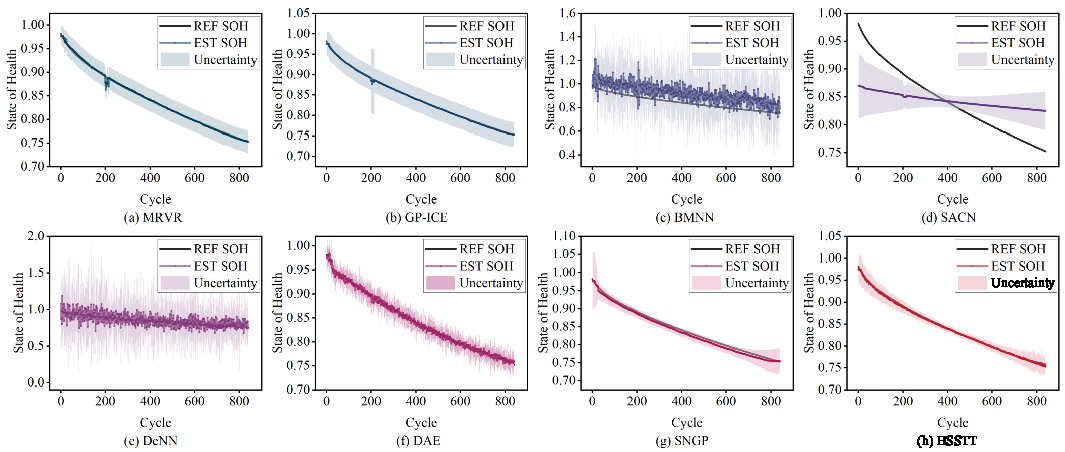
\includegraphics[width=6.5in]{figures/figure3/results.pdf}
\caption{TJU 数据集电池 26 的不确定性感知 SOH 估计结果。}
\label{fig:main_results}
\end{figure*}

% 所提出的 HSSTT 和其他基线模型的平均 SOH 估计、不确定性量化和校准结果呈现在表~\ref{tab:main-results} 中。总体而言，HSSTT 在所有方面均优于比较模型，且这种优越性能在所有数据集上都能观察到。相对于先前 SOTA 结果的改进值得注意。以 MIT 数据集为例，MAE、RMSE、NLL 和 ECE 的平均降低率分别为 18.10\%、9.88\%、23.48\% 和 40.26\%。
% % 具体而言，尽管 MRVR 和 GP-ICE 实现了相对较高的估计精度，但它们受限于模型容量和对数据分布的错误归纳偏差。它们的估计结果容易受到噪声影响并表现出强烈的不一致性，表明存在严重的模型校准错误，这不符合可信性的要求。DeNN 在一定程度上缓解了这个问题，但集成策略导致训练和部署的显著开销，阻碍了其在现实场景中的应用。类似地，BMNN 使用的 BBB 策略也导致大量计算开销。这种将 SOH 估计与不确定性量化紧密耦合的方法受输入特征分布稀疏性的影响很大，严重阻碍了准确的 SOH 估计。相反，SNGP 只需要一次前向传播即可估计输出后验分布的统计量。同样受输入信息稀疏性的影响，SNGP 容易产生不准确的 SOH 估计和不可靠的不确定性量化结果。BDAE 基于 MCD 实现不确定性量化。这些方法对超参数设置敏感，因此依赖于繁琐的参数搜索过程。上述所有方法都只关注退化过程中的时间相关性，忽视了传感器信号之间存在的空间相关性。SACN 通过利用胶囊网络提取时空信息来解决这一问题。然而，这种方法仍然难以应对稀疏性挑战，无法实现可信的 SOH 估计。HSSTT 充分考虑并解决了这些缺点，实现了可信的电池预测。
% % 为进一步阐明 HSSTT 的可信性，我们在图~\ref{fig:main_results} 中给出了 HSSTT 与其他基线在三个数据集上的定性结果。
% % 我们还在图~\ref{} 中提供了定性结果以进行演示。

% 表~\ref{tab:main-results} 中详细列出了所提出的 HSSTT 和基线模型的平均 SOH 估计以及不确定性量化和校准结果。HSSTT 在所有指标和数据集上一致优于比较模型，表现出优越的性能。值得注意的是，相对于先前最先进 SOTA 结果的增强是显著的。例如，对于 MIT 数据集，MAE、RMSE、NLL 和 ECE 的降低率分别为 18.10\%、9.88\%、23.48\% 和 40.26\%。此外，图~\ref{fig:main_results} 中显示了定性结果以供进一步演示。

表~\ref{tab:main-results} 中详细列出了所提出的 HSSTT 和基线模型的平均 SOH 估计以及不确定性量化和校准结果。HSSTT 在所有指标和数据集上一致优于比较模型，表现出优越的性能。值得注意的是，相对于先前最先进 SOTA 结果的增强是显著的。例如，对于 MIT 数据集，MAE、RMSE、NLL 和 ECE 的降低率分别为 18.10\%、9.88\%、23.48\% 和 40.26\%。此外，图~\ref{fig:main_results} 中显示了定性结果以供进一步演示。

此外，对各种模型进行了效率比较。MCDT\cite{20164903082858}、VIT\cite{20191806851746} 和 GSRT\cite{20193407356730} 代表三种使用不同策略的随机注意力机制。HSSTT 和基线模型的推理时间和存储利用率如表~\ref{tab:efficiency} 所示。HSSTT 不仅表现出卓越的估计精度和不确定性量化质量，而且实现了显著的计算效率，共同赋予其在工业系统中强大的实际应用性。

\newtext{为验证对 HSSTT 效率至关重要的聚类注意力模块，因此我们分析了其对延迟和模块内部机制的影响。如图~\ref{fig:clustered_attention}(a) 所示，与标准注意力基线相比，该模块显著降低了推理延迟。这种改进源于其通过将原始高维键投影到由学习质心定义的紧凑低维流形上来执行稀疏特征提取的能力，这一过程在图~\ref{fig:clustered_attention}(b) 中可视化。}

\begin{figure}[htbp]
  % \vspace{-1em}
  \centering
  \includegraphics[width=3.4in]{figures/clustered_attention_to_pdf.pdf}
  \caption{\newtext{所提出的聚类注意力机制的计算效率和稀疏化行为。}}
  \label{fig:clustered_attention}
  \end{figure}

% \begin{figure*}[ht]
% % \vspace{-1em}
% \centering
% 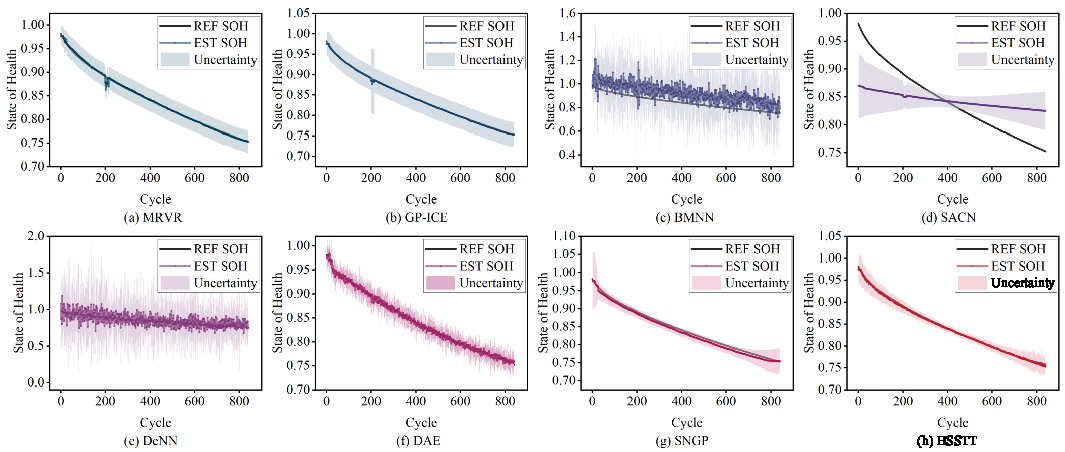
\includegraphics[width=6.5in]{figures/figure3/results.pdf}
% \caption{{TJU 数据集电池 26 的不确定性感知 SOH 估计结果。}}
% \label{fig:main_results}
% \end{figure*}

\begin{table}[htbp]
  % \color{blue}
\centering
\caption{计算效率比较结果}
\scalebox{0.8}
    {
      \small
  \begin{tabular}{cccc}
  \toprule
        模型 & \multicolumn{1}{l}{\makecell{推理\\延迟 (s)}} & \multicolumn{1}{l}{\makecell{内存\\使用 (MB)}} & \multicolumn{1}{l}{\makecell{平均\\RMSE}}\\
  \midrule
  MRVR  & 0.0149 & 1.2 & 0.067 \\
  GP-ICE & 0.0025 & 1.5 & 0.020 \\
  BMNN  & 0.0113 & 35.27 & 0.138 \\
  SACN  & 0.024 & 23.3 & 0.037 \\
  DeNN  & 0.0296 & 250 & 0.058 \\
  BDAE  & 0.0536 & 73.4 & 0.081 \\
  SNGP  & 0.0702 & 56.5 & 0.051 \\
  MCDT & 0.0316 & 35.3 & 0.138 \\
  VIT & 0.0124 & 20.3 & 0.026 \\
  GSRT & 0.0106 & 20.5 & 0.057 \\
  HSSTT & 0.0139 & 21.5 & 0.018 \\
  \bottomrule
  \end{tabular}%
    }
% \vspace{-0.5em}
\label{tab:efficiency}%
\end{table}

\subsection{消融研究}\label{subsec:ablation_study}

% 进行消融研究以解决以下问题：GSR 和 MCD 策略之间的区别、时空退化特征表示的影响以及分层自注意力的影响。缺少特定组件的 HSSTT 变体详见表~\ref{tab:ablation_study_1}。
进行消融研究以解决以下问题：GSR 与替代随机自注意力构建策略之间的区别、时空退化特征表示的影响以及分层自注意力的影响。缺少特定组件的 HSSTT 变体详见表~\ref{tab:ablation_study_1}。
% 首先，我们观察到用基于 MCD 的随机 Transformer 替换基于 GSR 的随机 Transformer 后，RMSE 和 NLL 显著下降，这证明了 GSR 策略在 SOH 估计精度和不确定性量化能力方面优于 MCD 策略。此外，通过分别从 HSSTT 中移除分层注意力机制和时空特征提取器，预测精度和不确定性量化质量也降低了，证明分层时空特征提取器增强了模型表示低秩 MTS 信号的能力。
此外，我们探索了校准对模型的影响，利用 ECE 和校准曲线对校准效果进行定量和定性评估。如表~\ref{tab:ablation_study_2} 和图~\ref{fig:calibration} 所示，校准后的 HSSTT 平均 ECE 降低 64.1\% 证明了所提出校准策略的有效性。这一改进进一步得到校准图的证实，其中校准后的曲线接近理想曲线，显著缓解了置信度不足或过高的问题。

\begin{table}[!t]
  % \vspace*{-2em}
    \centering
    \caption{HSSTT 消融研究结果}
    \resizebox{\linewidth}{!}
      {
      % \scalebox{0.8}
      % {
      %   \small
    \begin{threeparttable}
      
        \begin{tabular}{ccccccccc}
      \toprule
      数据集 & \multicolumn{2}{c}{MIT} & \multicolumn{2}{c}{TRI} & \multicolumn{2}{c}{TJU} & \multicolumn{2}{c}{{XJTU}} \\
      \cmidrule{2-9} 指标 & RMSE  & NLL   & RMSE  & NLL   & RMSE  & NLL & {RMSE}  & {NLL} \\
      \midrule
      MCDT\tnote{a} & 0.181  & 6.176  & 0.168  & 4.904  & 0.019  & 1.212 & {0.186} & {185.139} \\
      GSRT\tnote{b} & 0.062 & 1.188 & 0.065 & -0.767 & 0.011 & -3.158 & {0.088} & {3.731} \\
      {VIT\tnote{c}} & {0.040} & {4.723} & {0.033} & {4.736} & {0.004} & {3.868} & {0.028} & {14.713} \\
      {MCDL\tnote{d}} & {0.042} & {-1.093} & {0.046} & {1.604} & {0.009} & {-4.062} & {0.085} & {8.292}  \\
      {MCDACL\tnote{e}} & {0.045} & {70.386} & {0.036} & {43.768} & {0.007} & {-0.306} & {0.065} & {16.140} \\
      {MCDG\tnote{f}} & {0.056} & {10.118} & {0.031} & {4.662} & {0.009} & {-1.907} & {0.071} & {5.602} \\
      w/o S\tnote{{g}} & 0.041  & -0.883  & 0.032  & 1.659  & 0.005  & -4.311 & {0.031} & {-2.386} \\
      w/o T\tnote{{h}} & 0.038  & -1.444  & 0.031  & 0.483  & 0.004  & -4.461 & {0.035} & {-2.351}  \\
      HSSTT  & \textbf{0.029} & \textbf{-2.760} & \textbf{0.022} & \textbf{-2.966} & \textbf{0.003} & \textbf{-4.783} & {\textbf{0.016}} & {\textbf{-3.462}} \\
      \bottomrule
      \end{tabular}
      
      \begin{tablenotes}
        \item[{a, b, c}] {基于蒙特卡洛 dropout（MCD）\cite{20164903082858}、Gumbel-Softmax 重参数化（GSR）\cite{20193407356730} 和变分推理（VI）\cite{20191806851746} 的随机 Transformer。}
        \item[{d, e}] {基于 MCD 的 Vanilla LSTM\cite{sak2014long} 和 Auto-CNN-LSTM\cite{9137406}。}
        \item[{f}] {基于 MCD 的 CL-GraphSAGE\cite{YAO2023106437}。}
        \item[{g, h}] 移除注意力聚类（时间不确定性不感知）和重加权扩展卷积（空间不确定性不感知）。
    \end{tablenotes}
    
  \end{threeparttable}
  }
    \label{tab:ablation_study_1}%
  \end{table}%

\begin{figure}[!t]
  \centering
  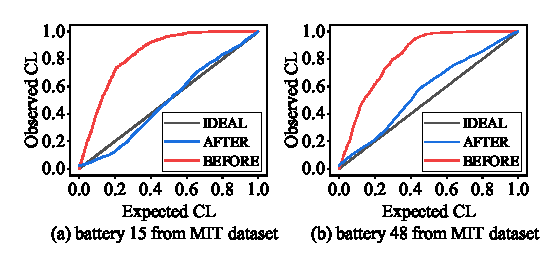
\includegraphics[width=3in]{figures/figure4/calibration.eps}
  \caption{校准前后曲线。横轴和纵轴分别表示估计和真实的置信水平。}
  % \vspace{-0.5em}
  \label{fig:calibration}
  \end{figure}

\begin{table}[h]
  % \vspace*{-2em}
  \centering
  % \caption{HSSTT 校准前后 ECE 评估}
  \caption{HSSTT 不确定性校准前后的期望校准误差（ECE）}
  \resizebox{\linewidth}{!}
    {
    % \scalebox{0.75}
    % {
    %   \small
      \begin{tabular}{ccccccccc}
    \toprule
    数据集 & \multicolumn{2}{c}{MIT} & \multicolumn{2}{c}{TRI} & \multicolumn{2}{c}{TJU} & \multicolumn{2}{c}{XJTU} \\
\cmidrule{2-9}    电池编号 & 校准前 & 校准后 & 校准前 & 校准后 & 校准前 & 校准后 & 校准前 & 校准后 \\
    \midrule
    1     & 14.599  & 7.648  & 29.990  & 11.252  & 20.634  & 18.533 & {37.259} & {6.625} \\
    2     & 33.470  & 3.000  & 35.485  & 14.635  & 11.581  & 3.933 & {38.051} & {8.310} \\
    3     & 28.117  & 13.658  & 26.886  & 11.297  & 29.622  & 17.762 & {36.083} & {12.198} \\
    4     & 22.686  & 11.815  & 22.819  & 14.271  & 41.214  & 6.136 & {39.084} & {15.253} \\
    5     & 32.069  & 6.650  & 30.502  & 10.614  & 36.668  & 14.158 & {40.430} & {15.020} \\
    6     & $\backslash$ & $\backslash$ & 23.887  & 12.210  & 41.497  & 13.941 & {40.292}  & {10.961} \\
    7     & $\backslash$ & $\backslash$ & 17.439  & 12.814  & 41.342  & 7.945 & {36.645} &  {13.172} \\
    8     & $\backslash$ & $\backslash$ & 41.527  & 9.065  & 40.247  & 9.318 & {29.393} &  {17.611} \\
    9     & $\backslash$ & $\backslash$ & $\backslash$ & $\backslash$ & 25.020  & 10.555 & {$\backslash$} & {$\backslash$} \\
    \midrule
    平均  & \multicolumn{2}{c}{26.188 $\to$ 8.554} & \multicolumn{2}{c}{28.567 $\to$ 12.020} & \multicolumn{2}{c}{31.980 $\to$ 11.365} & \multicolumn{2}{c}{{37.155 $\to$ 12.394}} \\
    \bottomrule
    \end{tabular}%
    }
  \label{tab:ablation_study_2}%
  % \vspace*{-2em}
\end{table}%

\begin{figure*}[ht]
  % \vspace{-1.5em}
\centering
\subfloat{
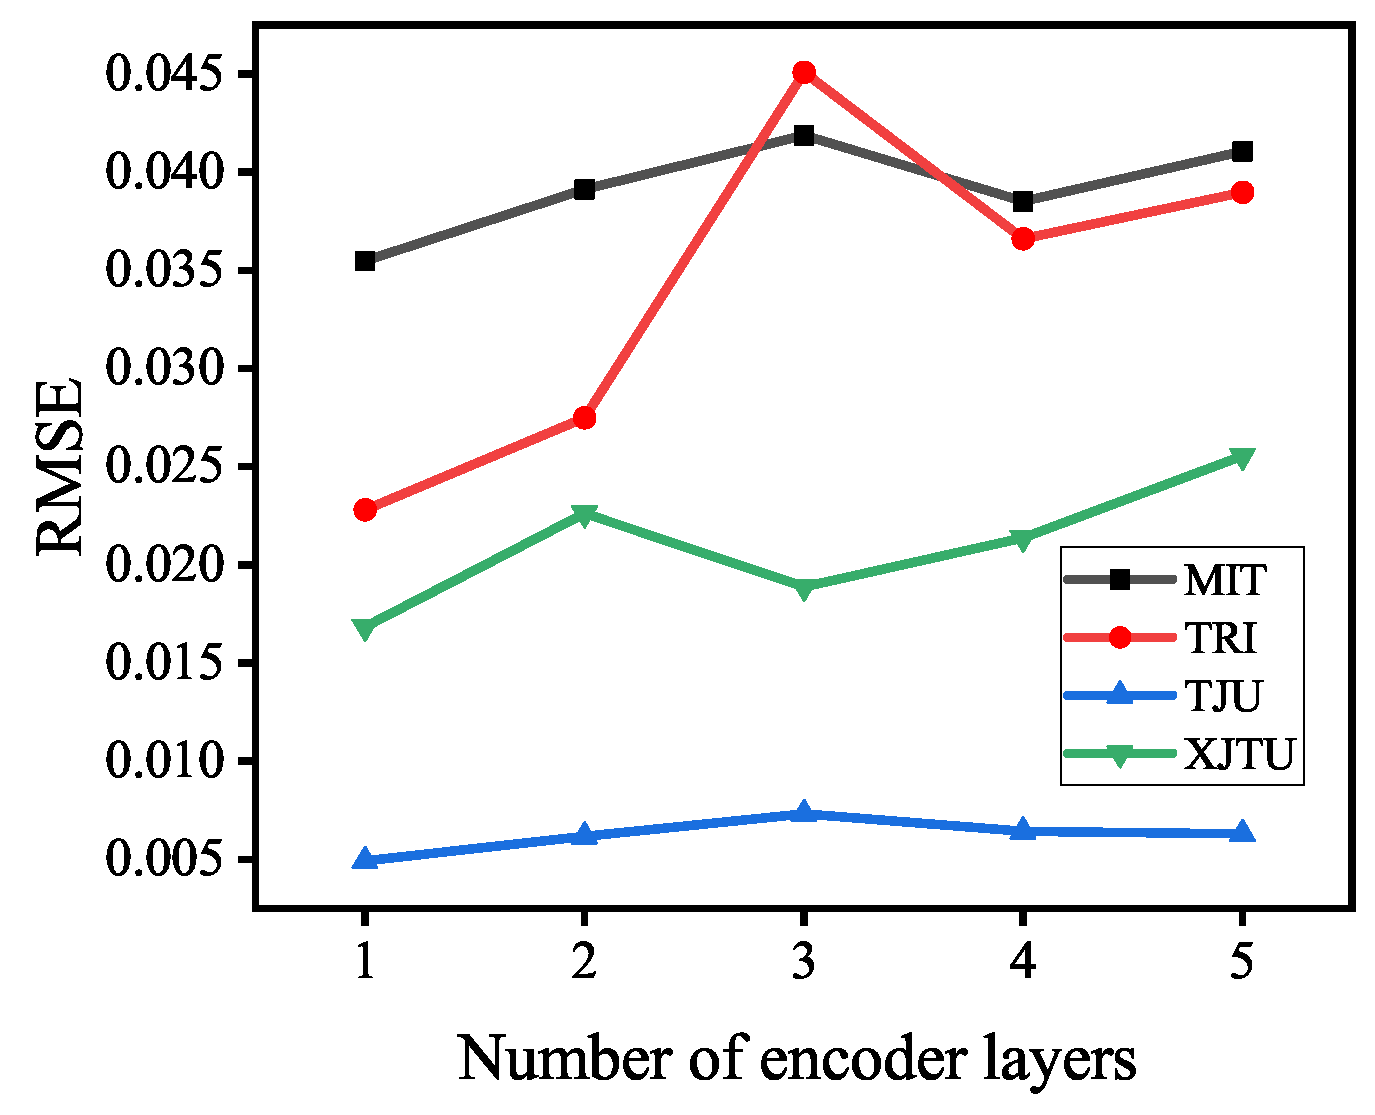
\includegraphics[width=1.6in]{figures/figurex/fig_layers.eps}
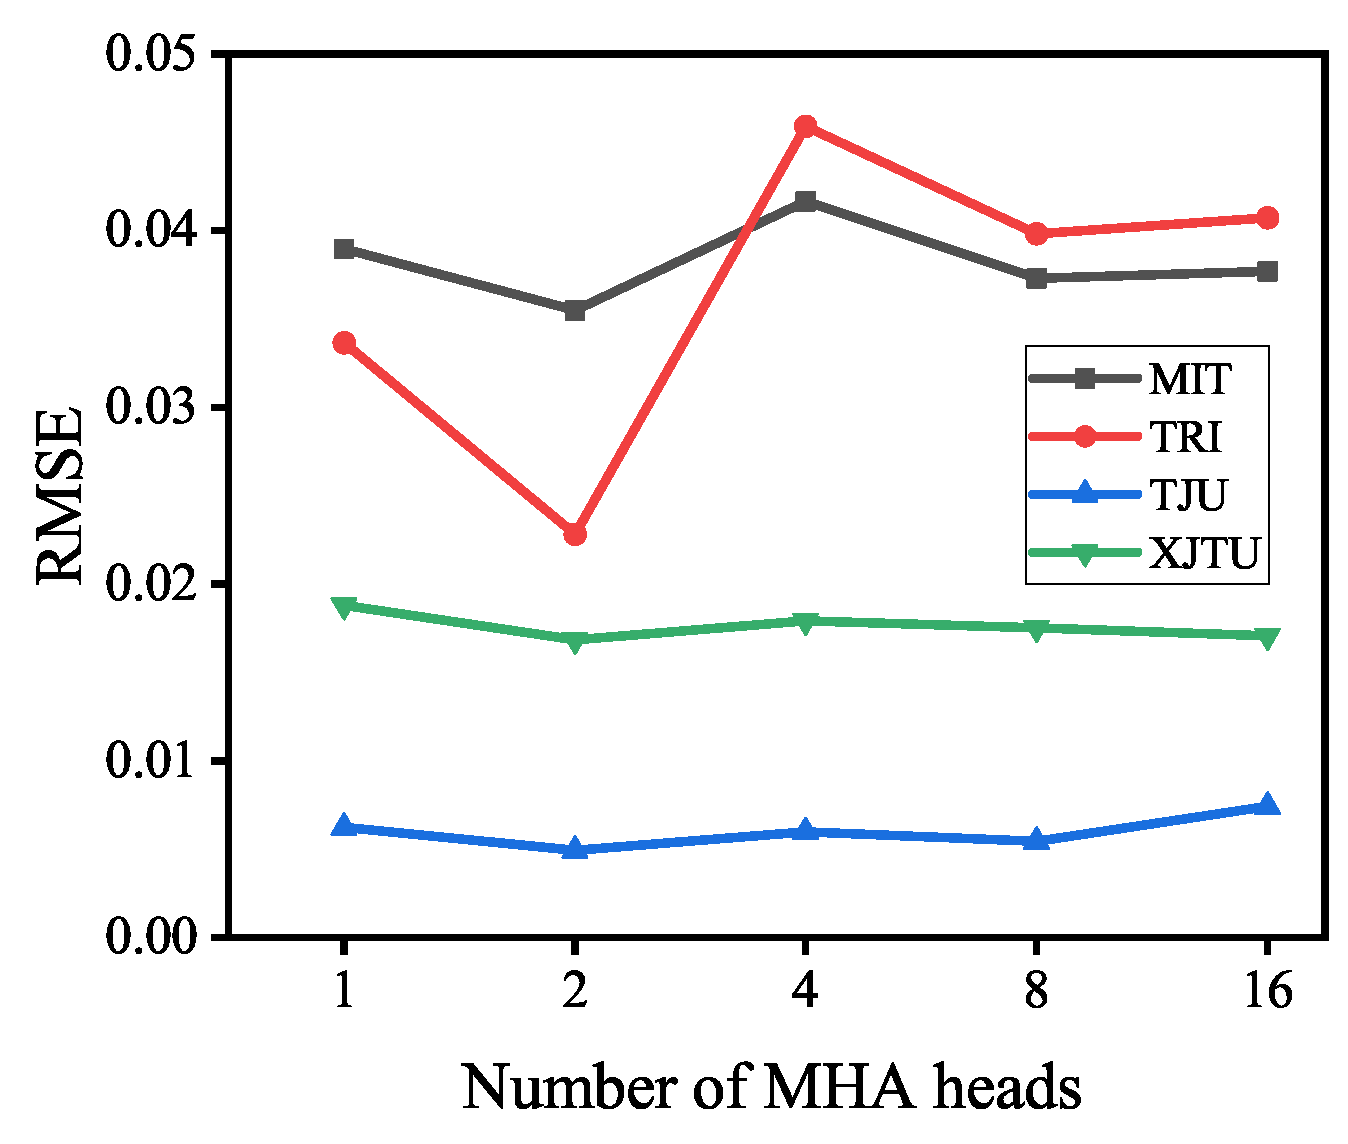
\includegraphics[width=1.6in]{figures/figurex/fig_heads.eps}
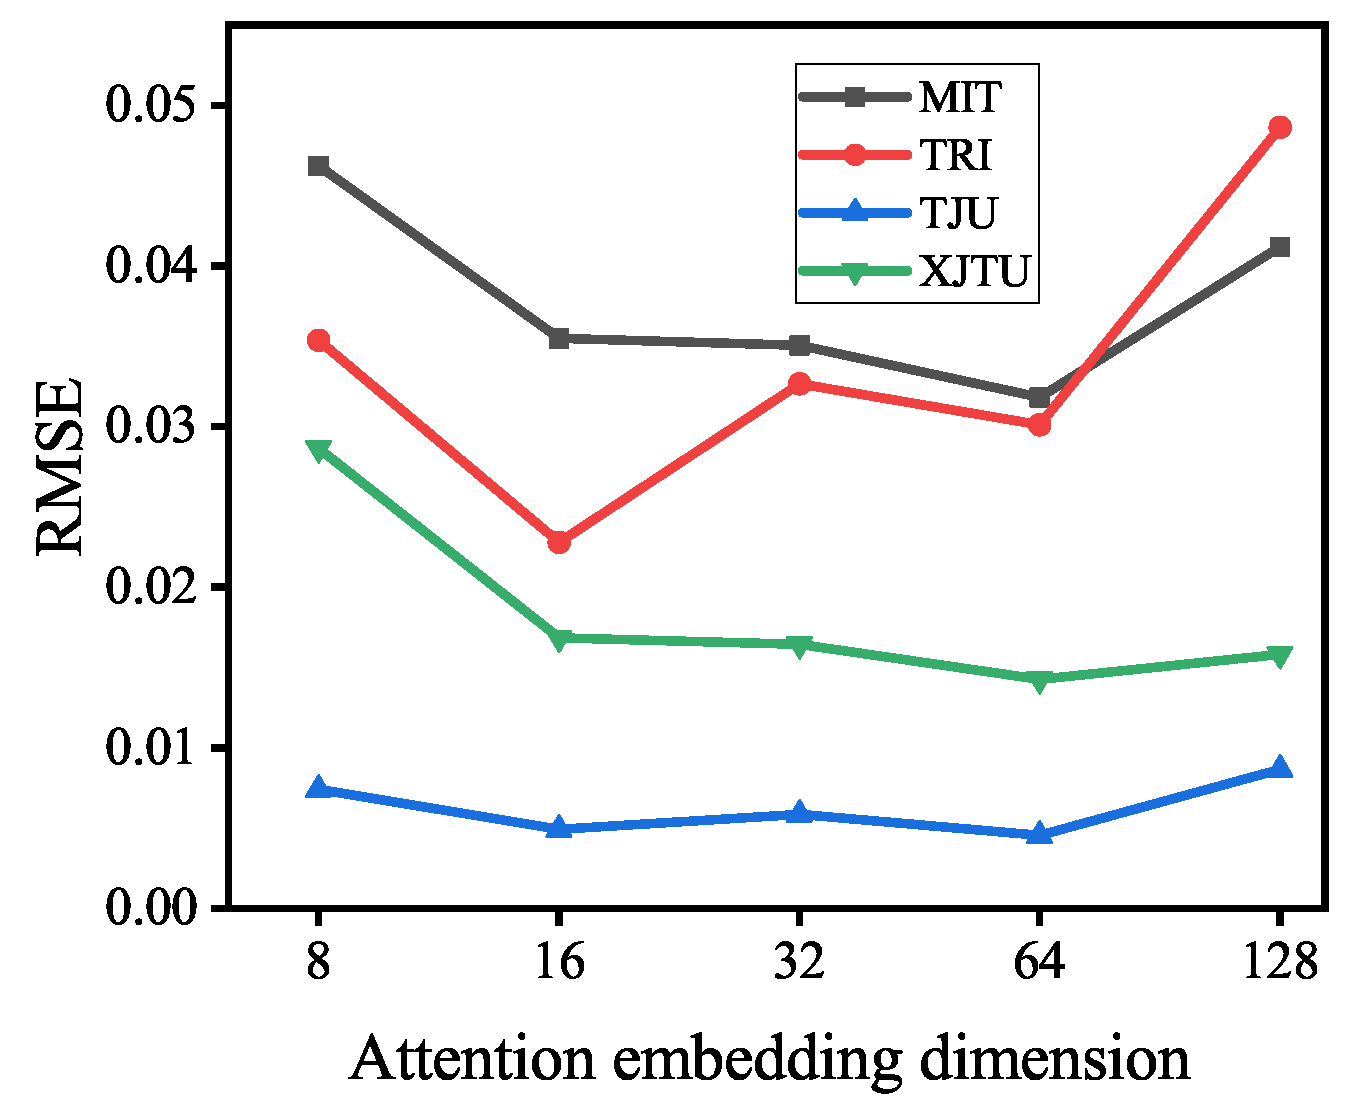
\includegraphics[width=1.6in]{figures/figurex/fig_dim.eps}
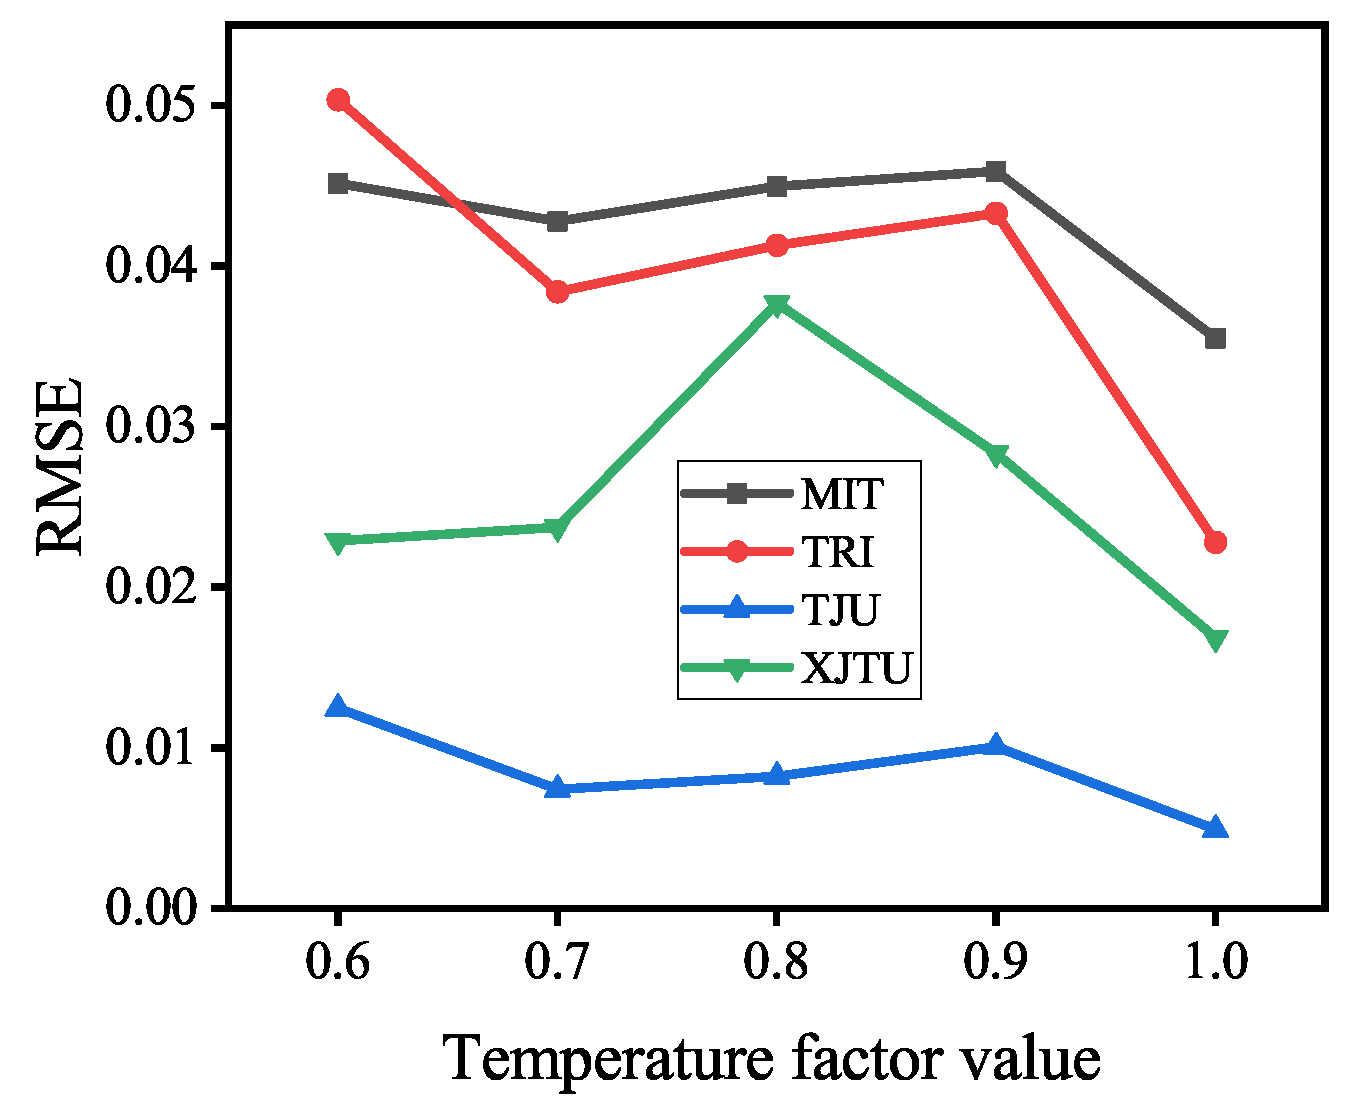
\includegraphics[width=1.6in]{figures/figurex/fig_tau.eps}
}
% \hfil
  % \vspace{0.5em}
\caption{HSSTT 在 MIT、TRI、TJU 和 XJTU 数据集上的超参数敏感性分析。}
\label{fig:hyperparameter}
\end{figure*}

\begin{table}[htbp]
  % \vspace{-0.5em}
    \centering
    % \caption{HSSTT 对 ID 和 OOD 样本的预测不确定性}
    \caption{HSSTT 对分布内（ID）和分布外（OOD）样本的预测不确定性}
    \scalebox{0.8}
    {
      \small
    \begin{threeparttable}
      \begin{tabular}{ccccc}
      \toprule
      数据集 & \multicolumn{2}{c}{分布内\tnote{a}} & \multicolumn{2}{c}{分布外\tnote{b}} \\
  \cmidrule{2-5} 电池编号 & 锐度 & NLL   & 锐度 & NLL \\
      \midrule
      1     & 0.021  & -2.047 & 0.059  & 5.180    \\
      2     & 0.024  & -3.421 & 0.047  & -1.752   \\
      3     & 0.023  & -3.010 & 0.053  & 11.448 \\
      4     & 0.028  & -1.862 & 0.062  & 2.787   \\
      5     & 0.023  & -3.463  & 0.048  & 17.378\\
      \midrule
      平均  & 0.024 & -2.760 & 0.054  & 7.008  \\
      \bottomrule
      \end{tabular}%
      \begin{tablenotes}
          \item[a] MIT $\to$ MIT
          \item[b] TRI $\to$ MIT
      \end{tablenotes}
      \end{threeparttable}
    \label{tab:id_ood}
    % \vspace*{-0.5em}
    }
  \end{table}%

\begin{figure}[t]
  \centering
  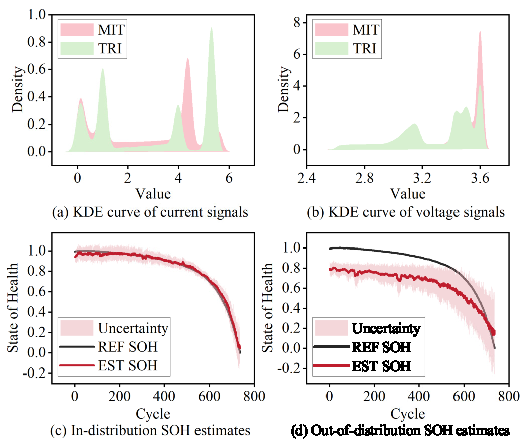
\includegraphics[width=3.in]{figures/figure5/ood.pdf}
  \caption{说明 MIT 和 TRI 数据集之间分布差异的示意图，以及 ID（MIT $\to$ MIT）和 OOD（TRI $\to$ MIT）样本的不确定性量化结果。}
  \label{fig:ood}
  % \vspace*{-1em}
  \end{figure}

\subsection{超参数敏感性分析}\label{subsec:sensitivity_analysis}

我们进行了敏感性分析以评估超参数对 HSSTT 性能的影响。这些超参数包括编码器层数 $n_{encoder}$、MHA 头数 $n_{head}$、注意力嵌入维度 $d_{emb}$ 和注意力温度因子 $\tau$（通过设置 $\tau_{1} = \tau_{2} = \tau$ 简化）。具体而言，我们为每个超参数设置以下值范围：$n_{encoder} \in \{1, 2, 3, 4, 5\}$、$n_{head} \in \{1, 2, 4, 8, 16\}$、$d_{emb} \in \{8, 16, 32, 64, 128\}$ 和 $\tau \in \{0.6, 0.7, 0.8, 0.9, 1.0\}$。分析在四个数据集上进行，使用 RMSE 作为评估指标。

如图~\ref{fig:hyperparameter} 所示，当 $n_{encoder} = 1$ 时，HSSTT 模型实现了其参数大小与问题规模之间的最佳对齐。类似地，设置 $n_{head} = 2$ 可产生最佳的子空间映射退化模式数量，而 $d_{emb} = 16$ 在性能和计算效率之间提供了理想的权衡。此外，$\tau = 1$ 使 HSSTT 模型中的注意力分数更平滑，增强了对时空退化模式的适应性。

\subsection{ID 与 OOD 样本的实验研究}\label{subsec:id_ood}

在本小节中，我们进行两项任务来评估 HSSTT 在 OOD 检测方面的性能。在\textit{任务 I} 中，训练和测试样本均来自 MIT 数据集，将测试样本归类为 ID。相反，在\textit{任务 II} 中，HSSTT 在 TRI 数据集上训练并在 MIT 数据集上测试，在此上下文中将 MIT 样本渲染为 OOD。我们使用锐度——定义为平均输出不确定性——和 NLL 来评估 HSSTT 的预测不确定性。结果呈现在表~\ref{tab:id_ood} 中，证明 HSSTT 对 ID 样本始终表现出较低的不确定性，对 OOD 样本表现出较高的不确定性，表明其能够基于预测不确定性有效识别 OOD 样本的能力，这是可信 SOH 估计的关键方面。

为清楚说明两个数据集上 ID-OOD 实验的设置，我们呈现了电压和电流信号核密度估计（KDE）曲线，如图~\ref{fig:ood}(a) 和 (b) 所示。这些曲线突出了由于充电和放电协议不同而导致的特征分布差异。随后，图~\ref{fig:ood}(c) 和 (d) 描述了 SOH 估计结果。值得注意的是，OOD 样本的估计区间明显比 ID 样本的区间宽，与先前所述结论一致。

\section{结论}\label{sec:conclusion}

在本文中，我们提出了用于可信 SOH 估计的 HSSTT。首先，我们设计了基于 Gumbel-Softmax 表示的随机自注意力以进行不确定性感知建模。
% 
其次，我们开发了分层 token 距离敏感 Transformer 编码器，并将其与跨传感器依赖性感知时间步卷积集成。这使得能够捕获循环数据中的时空动态并识别与退化相关的特征。
% 
第三，我们提出了一种有原则的回归器来纠正可能校准错误的不确定性，确保 LIBs 的可信 SOH 估计。全面的实验结果表明，HSSTT 在可信性方面优于现有方法，凸显了其优越性。

\newtext{尽管其性能前景广阔，但现代工业环境越来越需要可信的预测系统，这些系统能够在校准时不依赖大量独立同分布数据的情况下有效且高效地运行。因此，我们未来的工作将沿着两条互补的路径进行。首先，我们将专注于所提出框架在真实工业场景中的部署、测试和优化，以严格验证其实际有效性和鲁棒性。其次，为解决上述数据依赖性，我们的研究将更深入地研究基于不确定性的无源域自适应的固有挑战。}

\bibliographystyle{IEEEtran}
\bibliography{reference.bib}

% \begin{IEEEbiography}[{
\includegraphics[width=1in,height=1.25in,clip,keepaspectratio]{biography/fig1}}]{林新辉} 于 2023 年获得华北电力大学智能科学与技术学士学位。他目前正在东北大学攻读计算机科学与技术硕士学位。
    
% 他的研究兴趣包括预测与健康管理（PHM）、工业物联网（IIoT）和可解释人工智能（XAI）。
% \end{IEEEbiography}

\end{document}
